\begin{frame}[fragile]{Tutorial: One-site operators}

\begin{columns}

\begin{column}{4.5cm}

\begin{onlyenv}<1->
\begin{lstlisting}[language=JuliaLocal, style=julia, basicstyle=\scriptsize\ttfamily]
(dag(Zm)' * X * Zp)[]
inner(Zm', X, Zp)
\end{lstlisting}
\end{onlyenv}

\begin{onlyenv}<3->
~\\
\begin{lstlisting}[language=JuliaLocal, style=julia, basicstyle=\scriptsize\ttfamily]
apply(X, Zp) == 
  noprime(X * Zp)



inner(Zm, apply(X, Zp))
\end{lstlisting}
\end{onlyenv}

\end{column}

\begin{column}{4.5cm}

\begin{onlyenv}<1-1>
%\vspace*{-0.2cm}
$\langle Z-|X|Z+\rangle \approx 1$ \\
\end{onlyenv}

\begin{onlyenv}<3->
~\\
~\\
\end{onlyenv}

\begin{onlyenv}<2->
\vspace*{-0.2cm}
\begin{center}

\includegraphics[width=0.7\textwidth]{
  slides/assets/ZmXZp.png
}
\end{center}
\vspace*{0.0cm}
\end{onlyenv}

\begin{onlyenv}<3-3>
\vspace*{0.0cm}
~\\
$X|Z+\rangle$ \\
~\\
~\\
~\\
$\langle Z-|X|Z+\rangle \approx 1$ \\
~\\
\end{onlyenv}

\begin{onlyenv}<4->
\vspace*{0.2cm}
~\\
\begin{center}
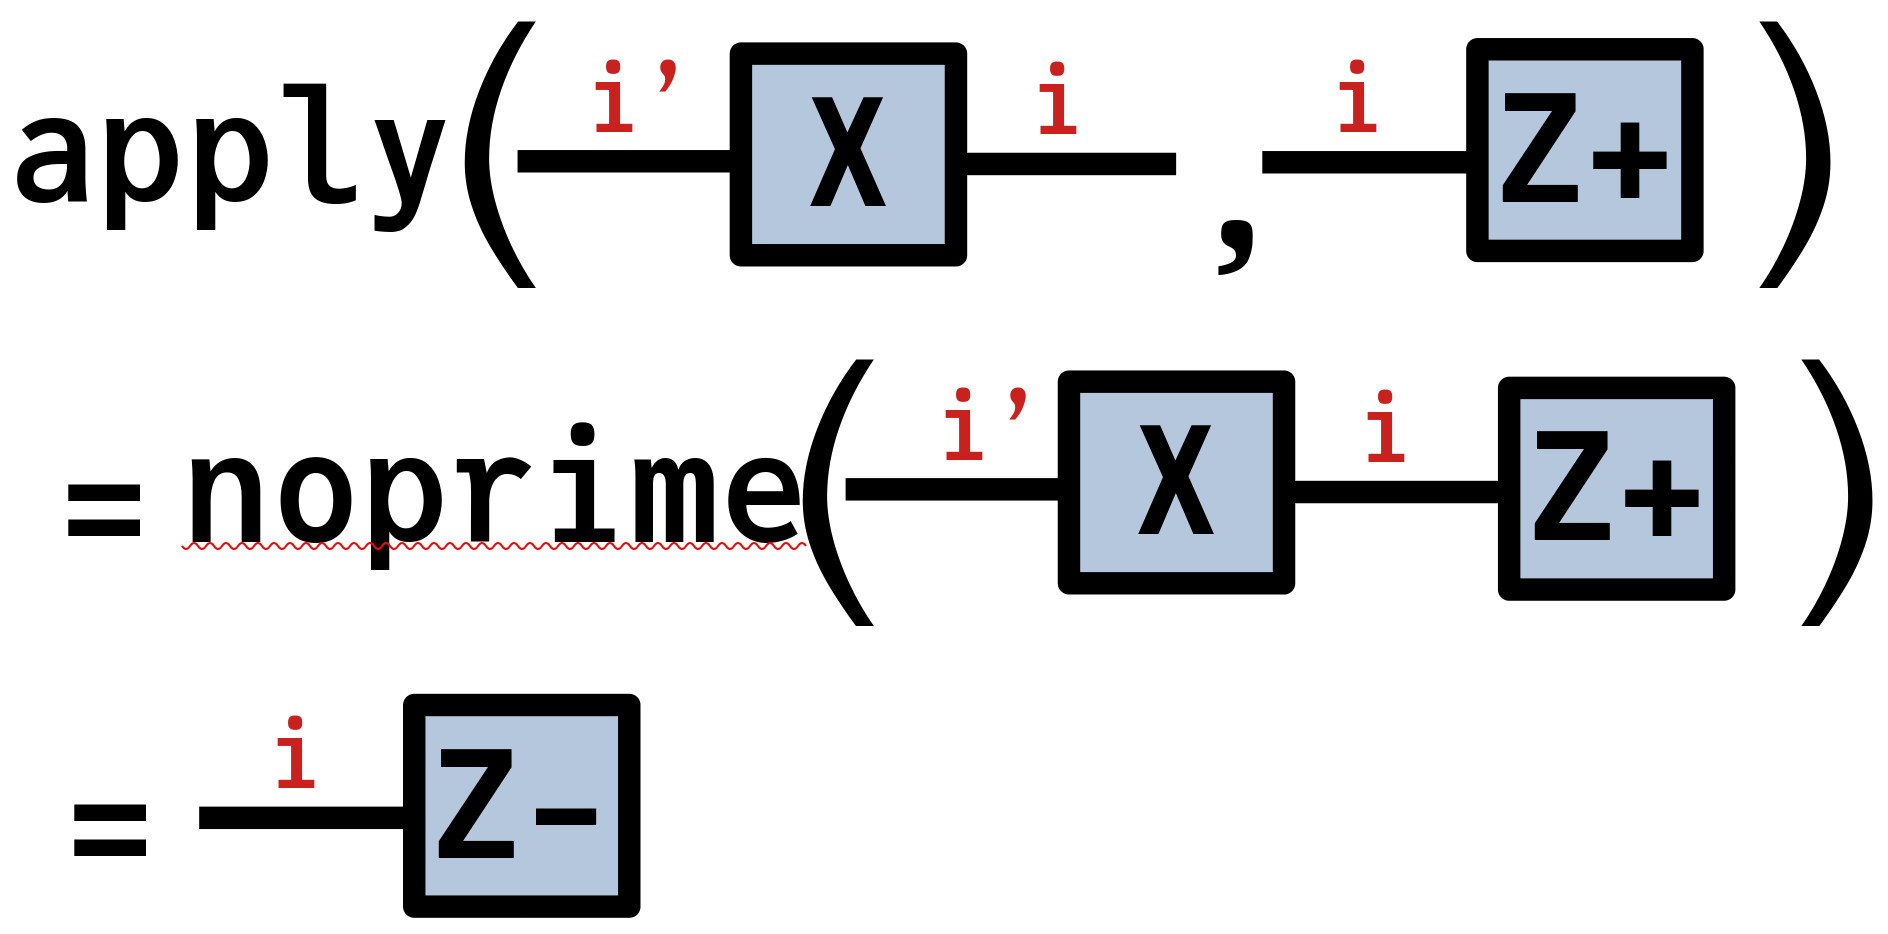
\includegraphics[width=1.0\textwidth]{
  slides/assets/apply_XZp.png
}
\end{center}
\vspace*{0.0cm}
\end{onlyenv}

\end{column}

\end{columns}

\end{frame}
